\section{OD requirements}

\begin{tcolorbox}[colback=red!5!white, colframe=red!50!black, title=Key Plots]
\begin{enumerate}
    \item Simulation Efficiency
    \item Neutron capture energy deposits
    \item alpha,n energies
    \item fraction of gammas that get captured in the OD after SS (AmLi sims)
    \item fraction of neutrons that get captured in each volume
    \item time spent in volume vs OD capture time (for all and for Gd-only) to show what causes each component
    \item Energy deposited in OD vs veto time
\end{enumerate}
\end{tcolorbox}

\par
As previously stated, the primary purpose of the OD is to act as an active veto for neutrons.
Practically, this means that there are a number of performance requirements which the OD has to meet, all of which can be found in \cite{LZ_TechnicalDesignReview_ref}.
A subset, which are address in this Thesis are presented in Table \ref{tab:veto_requirements}.

\begin{table}[!htbp]
    \centering
    \begin{tabular}{p{0.3\textwidth}p{0.6\textwidth}} %{ c | c {\textwidth} } 
    \hline
    {Requirement Number} & {Description} \\ \hline
    R-160001             & Detection efficiency of 95\% for a 1 MeV neutron that scatters once in the xenon \\
    R-160005             & Must not veto more than 5\% of the WIMP search live-time
    \end{tabular}
    \caption{Selection of the OD veto performance requirements. Adapted from Table 12.2.6 from \cite{LZ_TechnicalDesignReview_ref}}
    \label{tab:veto_requirements}
\end{table} 

\par
The veto method adopted by LZ is to act as a 'dumb' veto, as no attempt will be made to determine that cause of light seen in the OD.
This means that an event will be vetoed if the following two conditions are met;
\begin{enumerate}
    \item A pulse is seen with an energy above the veto threshold.
    \item The pulse is within the veto window.
\end{enumerate}
The two requirements in Table \ref{tab:veto_requirements} are clearly intertwined.
The veto window and threshold are primarily determined by the background rate in the OD in order to reduce the impact on live-time.
This does however need to be balanced to maintain a suitable veto efficiency.

\subsection{OD Backgrounds}
\par
A background in the OD is any event that is not what it was designed to detect and veto - so any event that is not a neutron or $\gamma$ that has scattered once in the TPC.
There are three significant sources of backgrounds are; Cavern-$\gamma$'s, impurities in the GdLS and other detector components.
Additionally, during data-taking electronic noise will contribute to the background rate, however this is not taken into account here. 

\subsubsection{GdLS impurities}
\par
In order to ascertain the rate of internal contaminants expected, a campaign was undertaken \cite{scotthaselschwardt_thesis_ref} to determine this expected rate.
The results from this are shown in table \ref{tab:gdls_assay_rates}.
The decay chains and associated sub-chains are shown in Figure \ref{fig:decay_chains}.

\par
One of the key outcomes of the screener campaign were the high ${}^{235}U$ rate.
As such, the method of doping the LS was altered, which aimed to reduce the contamination.
The expected rates from this are also shown in Table \ref{tab:gdls_assay_rates}.
However, as these were not screened the accuracy is unknown, but gives a 'best-case'.


\begin{table}[!htbp]
    \centering
    \begin{tabular}{c|c|c}
        \multirow{2}{*}{Isotope or Subchain}  &  \multicolumn{2}{c}{GdLS rates (mBq/kg)}      \\ 
                             &  LS Screener          & Improved Purification \\ \hline
        ${}^{238}U_{e}$      &  $< 1.04$             & $< 0.017$             \\ 
        ${}^{238}U_{m}$      &  $0.092\pm0.02$       & $0.010\pm0.004$       \\
        ${}^{235}U_{e}$      &  $0.011$              & $< 0.018$             \\
        ${}^{235}U_{l}$      &  $0.10\pm0.04$        & $< 0.012$             \\
        ${}^{232}Th_{e}$     &  $< 0.027$            & $< 0.0036$            \\
        ${}^{232}Th_{l}$     &  $< 0.020$            & $< 0.0030$            \\
        ${}^{40}K$           &  $< 0.22$             & $< 0.0092$            \\
        ${}^{138}La$         &  $< 0.0055$           & $< 0.0017$            \\
        ${}^{176}Lu$         &  $0.30\pm0.07$        & $0.0081\pm0.0018$     \\
        ${}^{152}{Gd}$       &  $1.61\pm0.08$        & $1.61\pm0.08$         \\
        ${}^{152}{Sm}$       &  $1.02\pm0.05$        & $1.02\pm0.05$         \\
        ${}^{14}{C14}$       &  $4.77\pm0.098$       & $4.77\pm0.098$ 
    \end{tabular}
    \caption{Activities of GdLS components during LS Screener testing and those projected from an improved purification technique. Values from Table 4.9 and 6.11 of \cite{scotthaselschwardt_thesis_ref}}
    \label{tab:gdls_assay_rates}
\end{table}

\newcommand{\nodewidth}{1cm}
\newcommand{\textnodewidth}{0.2cm}
\newcommand{\nodeminimumwidth}{30pt}
\newcommand{\nodespacing}{10pt}


\begin{landscape}
\begin{figure}
    \centering
\begin{tikzpicture}
  [node distance=0.05cm,text centered, thick]
  \tikzstyle{every node}=[font=\fontsize{5}{5}\selectfont]
 
    % For 3 chains, need 13 across
 \node[draw, circle, inner sep=0pt, text width=\nodewidth, minimum width=\nodeminimumwidth, ] (uranium_node_0) {${}^{234}_{92}$U $245e^{3}$y};
 \node[circle, inner sep=0pt, text width=\nodewidth, minimum width=\nodeminimumwidth, right=of uranium_node_0] (uranium_node_1) {};
 \node[draw, circle, inner sep=0pt, text width=\nodewidth, minimum width=\nodeminimumwidth, right=of uranium_node_1] (uranium_node_2) {${}^{238}_{92}$U $4.5e^{9}$y};
 \node[circle, inner sep=0pt, text width=\nodewidth, minimum width=\nodeminimumwidth, right=of uranium_node_2] (uranium_node_3) {};
 \node[circle, inner sep=0pt, text width=\nodewidth, minimum width=\nodeminimumwidth, right=of uranium_node_3] (uranium_node_4) {};
 \node[circle, inner sep=0pt, text width=\nodewidth, minimum width=\nodeminimumwidth, right=of uranium_node_4] (chain_sep_1) {};
 \node[draw, circle, inner sep=0pt, text width=\nodewidth, minimum width=\nodeminimumwidth, right=of chain_sep_1] (uranium_node_5) {${}^{235}_{92}$U $7.0e^{8}$y};
 \node[circle, inner sep=0pt, text width=\nodewidth, minimum width=\nodeminimumwidth, right=of uranium_node_5] (uranium_node_6) {};
 \node[circle, inner sep=0pt, text width=\nodewidth, minimum width=\nodeminimumwidth, right=of uranium_node_6] (uranium_node_7) {};
 \node[circle, inner sep=0pt, text width=\nodewidth, minimum width=\nodeminimumwidth, right=of uranium_node_7] (uranium_node_8) {};
 \node[circle, inner sep=0pt, text width=\nodewidth, minimum width=\nodeminimumwidth, right=of uranium_node_8] (uranium_node_9) {};
 \node[circle, inner sep=0pt, text width=\nodewidth, minimum width=\nodeminimumwidth, right=of uranium_node_9] (chain_sep_2) {};
 \node[circle, inner sep=0pt, text width=\nodewidth, minimum width=\nodeminimumwidth, right=of chain_sep_2] (uranium_node_10) {};
 \node[circle, inner sep=0pt, text width=\nodewidth, minimum width=\nodeminimumwidth, right=of uranium_node_10] (uranium_node_11) {};
 \node[circle, inner sep=0pt, text width=\nodewidth, minimum width=\nodeminimumwidth, right=of uranium_node_11] (uranium_node_12) {};
 \node[circle, inner sep=0pt, text width=\nodewidth, minimum width=\nodeminimumwidth, right=of uranium_node_12] (uranium_label_sep) {};
 \node[circle, inner sep=0pt, text width=\nodewidth, minimum width=\nodeminimumwidth, right=of uranium_label_sep] (uranium_sep_3) {Uranium};
 
 \node[circle, inner sep=0pt, text width=\nodewidth, minimum width=\nodeminimumwidth, below=of uranium_node_0] (protactinium_node_0) {};
 \node[draw, circle, inner sep=0pt, text width=\nodewidth, minimum width=\nodeminimumwidth, below=of uranium_node_1] (protactinium_node_1) {${}^{234}_{91}$Pa $1.2$m};
 \node[circle, inner sep=0pt, text width=\nodewidth, minimum width=\nodeminimumwidth, below=of uranium_node_2] (protactinium_node_2) {};
 \node[circle, inner sep=0pt, text width=\nodewidth, minimum width=\nodeminimumwidth, below=of uranium_node_3] (protactinium_node_3) {};
 \node[circle, inner sep=0pt, text width=\nodewidth, minimum width=\nodeminimumwidth, below=of uranium_node_4] (protactinium_node_4) {};
 \node[circle, inner sep=0pt, text width=\nodewidth, minimum width=\nodeminimumwidth, below=of uranium_node_5] (protactinium_node_5) {};
 \node[draw, circle, inner sep=0pt, text width=\nodewidth, minimum width=\nodeminimumwidth, below=of uranium_node_6] (protactinium_node_6) {${}^{231}_{91}$Pa $3.3e^{4}$y};
 \node[circle, inner sep=0pt, text width=\nodewidth, minimum width=\nodeminimumwidth, below=of uranium_node_7] (protactinium_node_7) {};
 \node[circle, inner sep=0pt, text width=\nodewidth, minimum width=\nodeminimumwidth, below=of uranium_node_8] (protactinium_node_8) {};
 \node[circle, inner sep=0pt, text width=\nodewidth, minimum width=\nodeminimumwidth, below=of uranium_node_9] (protactinium_node_9) {};
 \node[circle, inner sep=0pt, text width=\nodewidth, minimum width=\nodeminimumwidth, below=of uranium_node_10] (protactinium_node_10) {};
 \node[circle, inner sep=0pt, text width=\nodewidth, minimum width=\nodeminimumwidth, below=of uranium_node_11] (protactinium_node_11) {};
 \node[circle, inner sep=0pt, text width=\nodewidth, minimum width=\nodeminimumwidth, below=of uranium_node_12] (protactinium_node_12) {};
 \node[circle, inner sep=0pt, text width=\nodewidth, minimum width=\nodeminimumwidth, below=of uranium_sep_3] (protactinium_sep_3) {Protactinium};
 
 \node[draw, circle, inner sep=0pt, text width=\nodewidth, minimum width=\nodeminimumwidth, below=of protactinium_node_0] (thorium_node_0) {${}^{230}_{90}$Th $75e^{3}$y};
 \node[circle, inner sep=0pt, text width=\nodewidth, minimum width=\nodeminimumwidth, below=of protactinium_node_1] (thorium_node_1) {};
 \node[draw, circle, inner sep=0pt, text width=\nodewidth, minimum width=\nodeminimumwidth, below=of protactinium_node_2] (thorium_node_2) {${}^{234}_{90}$Th $24.1$d};
 \node[circle, inner sep=0pt, text width=\nodewidth, minimum width=\nodeminimumwidth, below=of protactinium_node_3] (thorium_node_3) {};
 \node[circle, inner sep=0pt, text width=\nodewidth, minimum width=\nodeminimumwidth, below=of protactinium_node_4] (thorium_node_4) {};
 \node[draw, circle, inner sep=0pt, text width=\nodewidth, minimum width=\nodeminimumwidth, below=of protactinium_node_5] (thorium_node_5) {${}^{231}_{90}$Th $25.5$h};
 \node[circle, inner sep=0pt, text width=\nodewidth, minimum width=\nodeminimumwidth, below=of protactinium_node_6] (thorium_node_6) {};
 \node[draw, circle, inner sep=0pt, text width=\nodewidth, minimum width=\nodeminimumwidth, below=of protactinium_node_7] (thorium_node_7) {${}^{227}_{90}$Th $18.7$d};
 \node[circle, inner sep=0pt, text width=\nodewidth, minimum width=\nodeminimumwidth, below=of protactinium_node_8] (thorium_node_8) {};
 \node[circle, inner sep=0pt, text width=\nodewidth, minimum width=\nodeminimumwidth, below=of protactinium_node_9] (thorium_node_9) {};
 \node[draw, circle, inner sep=0pt, text width=\nodewidth, minimum width=\nodeminimumwidth, below=of protactinium_node_10] (thorium_node_10) {${}^{228}_{90}$Th $1.9$y};
 \node[circle, inner sep=0pt, text width=\nodewidth, minimum width=\nodeminimumwidth, below=of protactinium_node_11] (thorium_node_11) {};
 \node[draw, circle, inner sep=0pt, text width=\nodewidth, minimum width=\nodeminimumwidth, below=of protactinium_node_12] (thorium_node_12) {${}^{232}_{90}$Th $1.4e^{10}$y};
 \node[circle, inner sep=0pt, text width=\nodewidth, minimum width=\nodeminimumwidth, below=of protactinium_sep_3] (thorium_sep_3) {Thorium};
 
 \node[circle, inner sep=0pt, text width=\nodewidth, minimum width=\nodeminimumwidth, below=of thorium_node_0] (actinium_node_0) {};
 \node[circle, inner sep=0pt, text width=\nodewidth, minimum width=\nodeminimumwidth, below=of thorium_node_1] (actinium_node_1) {};
 \node[circle, inner sep=0pt, text width=\nodewidth, minimum width=\nodeminimumwidth, below=of thorium_node_2] (actinium_node_2) {};
 \node[circle, inner sep=0pt, text width=\nodewidth, minimum width=\nodeminimumwidth, below=of thorium_node_3] (actinium_node_3) {};
 \node[circle, inner sep=0pt, text width=\nodewidth, minimum width=\nodeminimumwidth, below=of thorium_node_4] (actinium_node_4) {};
 \node[circle, inner sep=0pt, text width=\nodewidth, minimum width=\nodeminimumwidth, below=of thorium_node_5] (actinium_node_5) {};
 \node[draw, circle, inner sep=0pt, text width=\nodewidth, minimum width=\nodeminimumwidth, below=of thorium_node_6] (actinium_node_6) {${}^{227}_{89}$Ac $21.8$y};
 \node[circle, inner sep=0pt, text width=\nodewidth, minimum width=\nodeminimumwidth, below=of thorium_node_7] (actinium_node_7) {};
 \node[circle, inner sep=0pt, text width=\nodewidth, minimum width=\nodeminimumwidth, below=of thorium_node_8] (actinium_node_8) {};
 \node[circle, inner sep=0pt, text width=\nodewidth, minimum width=\nodeminimumwidth, below=of thorium_node_9] (actinium_node_9) {};
 \node[circle, inner sep=0pt, text width=\nodewidth, minimum width=\nodeminimumwidth, below=of thorium_node_10] (actinium_node_10) {};
 \node[draw, circle, inner sep=0pt, text width=\nodewidth, minimum width=\nodeminimumwidth, below=of thorium_node_11] (actinium_node_11) {${}^{228}_{89}$Ac $6.1$h};
 \node[circle, inner sep=0pt, text width=\nodewidth, minimum width=\nodeminimumwidth, below=of thorium_node_12] (actinium_node_12) {};
 \node[circle, inner sep=0pt, text width=\nodewidth, minimum width=\nodeminimumwidth, below=of thorium_sep_3] (actinium_sep_3) {Actinium}; 
 
 \node[draw, circle, inner sep=0pt, text width=\nodewidth, minimum width=\nodeminimumwidth, below=of actinium_node_0] (radium_node_0) {${}^{226}_{89}$Ra $1.6e^{3}$y};
 \node[circle, inner sep=0pt, text width=\nodewidth, minimum width=\nodeminimumwidth, below=of actinium_node_1] (radium_node_1) {};
 \node[circle, inner sep=0pt, text width=\nodewidth, minimum width=\nodeminimumwidth, below=of actinium_node_2] (radium_node_2) {};
 \node[circle, inner sep=0pt, text width=\nodewidth, minimum width=\nodeminimumwidth, below=of actinium_node_3] (radium_node_3) {};
 \node[circle, inner sep=0pt, text width=\nodewidth, minimum width=\nodeminimumwidth, below=of actinium_node_4] (radium_node_4) {};
 \node[circle, inner sep=0pt, text width=\nodewidth, minimum width=\nodeminimumwidth, below=of actinium_node_5] (radium_node_5) {};
 \node[circle, inner sep=0pt, text width=\nodewidth, minimum width=\nodeminimumwidth, below=of actinium_node_6] (radium_node_6) {};
 \node[draw, circle, inner sep=0pt, text width=\nodewidth, minimum width=\nodeminimumwidth, below=of actinium_node_7] (radium_node_7) {${}^{223}_{88}$Ra $11.4$d};
 \node[circle, inner sep=0pt, text width=\nodewidth, minimum width=\nodeminimumwidth, below=of actinium_node_8] (radium_node_8) {};
 \node[circle, inner sep=0pt, text width=\nodewidth, minimum width=\nodeminimumwidth, below=of actinium_node_9] (radium_node_9) {};
 \node[draw, circle, inner sep=0pt, text width=\nodewidth, minimum width=\nodeminimumwidth, below=of actinium_node_10] (radium_node_10) {${}^{224}_{88}$Ra $3.6$d};
 \node[circle, inner sep=0pt, text width=\nodewidth, minimum width=\nodeminimumwidth, below=of actinium_node_11] (radium_node_11) {};
 \node[draw, circle, inner sep=0pt, text width=\nodewidth, minimum width=\nodeminimumwidth, below=of actinium_node_12] (radium_node_12) {${}^{228}_{88}$Ra $5.7$y};
 \node[circle, inner sep=0pt, text width=\nodewidth, minimum width=\nodeminimumwidth, below=of actinium_sep_3] (radium_sep_3) {Radium}; 
 
 \node[circle, inner sep=0pt, text width=\nodewidth, minimum width=\nodeminimumwidth, below=of radium_node_0] (francium_node_0) {};
 \node[circle, inner sep=0pt, text width=\nodewidth, minimum width=\nodeminimumwidth, below=of radium_node_1] (francium_node_1) {};
 \node[circle, inner sep=0pt, text width=\nodewidth, minimum width=\nodeminimumwidth, below=of radium_node_2] (francium_node_2) {};
 \node[circle, inner sep=0pt, text width=\nodewidth, minimum width=\nodeminimumwidth, below=of radium_node_3] (francium_node_3) {};
 \node[circle, inner sep=0pt, text width=\nodewidth, minimum width=\nodeminimumwidth, below=of radium_node_4] (francium_node_4) {};
 \node[circle, inner sep=0pt, text width=\nodewidth, minimum width=\nodeminimumwidth, below=of radium_node_5] (francium_node_5) {};
 \node[draw, circle, inner sep=0pt, text width=\nodewidth, minimum width=\nodeminimumwidth, below=of radium_node_6] (francium_node_6) {${}^{223}_{87}$Fr $22.0$m};
 \node[circle, inner sep=0pt, text width=\nodewidth, minimum width=\nodeminimumwidth, below=of radium_node_7] (francium_node_7) {};
 \node[circle, inner sep=0pt, text width=\nodewidth, minimum width=\nodeminimumwidth, below=of radium_node_8] (francium_node_8) {};
 \node[circle, inner sep=0pt, text width=\nodewidth, minimum width=\nodeminimumwidth, below=of radium_node_9] (francium_node_9) {};
 \node[circle, inner sep=0pt, text width=\nodewidth, minimum width=\nodeminimumwidth, below=of radium_node_10] (francium_node_10) {};
 \node[circle, inner sep=0pt, text width=\nodewidth, minimum width=\nodeminimumwidth, below=of radium_node_11] (francium_node_11) {};
 \node[circle, inner sep=0pt, text width=\nodewidth, minimum width=\nodeminimumwidth, below=of radium_node_12] (francium_node_12) {};
 \node[circle, inner sep=0pt, text width=\nodewidth, minimum width=\nodeminimumwidth, below=of radium_sep_3] (francium_sep_3) {Francium}; 
 
 \node[draw, circle, inner sep=0pt, text width=\nodewidth, minimum width=\nodeminimumwidth, below=of francium_node_0] (radon_node_0) {${}^{222}_{86}$Rn $3.8$d};
 \node[circle, inner sep=0pt, text width=\nodewidth, minimum width=\nodeminimumwidth, below=of francium_node_1] (radon_node_1) {};
 \node[circle, inner sep=0pt, text width=\nodewidth, minimum width=\nodeminimumwidth, below=of francium_node_2] (radon_node_2) {};
 \node[circle, inner sep=0pt, text width=\nodewidth, minimum width=\nodeminimumwidth, below=of francium_node_3] (radon_node_3) {};
 \node[circle, inner sep=0pt, text width=\nodewidth, minimum width=\nodeminimumwidth, below=of francium_node_4] (radon_node_4) {};
 \node[circle, inner sep=0pt, text width=\nodewidth, minimum width=\nodeminimumwidth, below=of francium_node_5] (radon_node_5) {};
 \node[circle, inner sep=0pt, text width=\nodewidth, minimum width=\nodeminimumwidth, below=of francium_node_6] (radon_node_6) {};
 \node[draw, circle, inner sep=0pt, text width=\nodewidth, minimum width=\nodeminimumwidth, below=of francium_node_7] (radon_node_7) {${}^{219}_{86}$Rn $4.0$s};
 \node[circle, inner sep=0pt, text width=\nodewidth, minimum width=\nodeminimumwidth, below=of francium_node_8] (radon_node_8) {};
 \node[circle, inner sep=0pt, text width=\nodewidth, minimum width=\nodeminimumwidth, below=of francium_node_9] (radon_node_9) {};
 \node[draw, circle, inner sep=0pt, text width=\nodewidth, minimum width=\nodeminimumwidth, below=of francium_node_10] (radon_node_10) {${}^{220}_{86}$Rn $55$s};
 \node[circle, inner sep=0pt, text width=\nodewidth, minimum width=\nodeminimumwidth, below=of francium_node_11] (radon_node_11) {};
 \node[circle, inner sep=0pt, text width=\nodewidth, minimum width=\nodeminimumwidth, below=of francium_node_12] (radon_node_12) {};
 \node[circle, inner sep=0pt, text width=\nodewidth, minimum width=\nodeminimumwidth, below=of francium_sep_3] (radon_sep_3) {Radon}; 
 
 \node[circle, inner sep=0pt, text width=\nodewidth, minimum width=\nodeminimumwidth, below=of radon_node_0] (astatine_node_0) {};
 \node[draw, circle, inner sep=0pt, text width=\nodewidth, minimum width=\nodeminimumwidth, below=of radon_node_1] (astatine_node_1) {${}^{218}_{85}$At $1.5$s};
 \node[circle, inner sep=0pt, text width=\nodewidth, minimum width=\nodeminimumwidth, below=of radon_node_2] (astatine_node_2) {};
 \node[circle, inner sep=0pt, text width=\nodewidth, minimum width=\nodeminimumwidth, below=of radon_node_3] (astatine_node_3) {};
 \node[circle, inner sep=0pt, text width=\nodewidth, minimum width=\nodeminimumwidth, below=of radon_node_4] (astatine_node_4) {};
 \node[circle, inner sep=0pt, text width=\nodewidth, minimum width=\nodeminimumwidth, below=of radon_node_5] (astatine_node_5) {};
 \node[draw, circle, inner sep=0pt, text width=\nodewidth, minimum width=\nodeminimumwidth, below=of radon_node_6] (astatine_node_6) {${}^{219}_{85}$At $56$s};
 \node[circle, inner sep=0pt, text width=\nodewidth, minimum width=\nodeminimumwidth, below=of radon_node_7] (astatine_node_7) {};
 \node[draw, circle, inner sep=0pt, text width=\nodewidth, minimum width=\nodeminimumwidth, below=of radon_node_8] (astatine_node_8) {${}^{215}_{85}$At $1e^{-4}$s};
 \node[circle, inner sep=0pt, text width=\nodewidth, minimum width=\nodeminimumwidth, below=of radon_node_9] (astatine_node_9) {};
 \node[circle, inner sep=0pt, text width=\nodewidth, minimum width=\nodeminimumwidth, below=of radon_node_10] (astatine_node_10) {};
 \node[circle, inner sep=0pt, text width=\nodewidth, minimum width=\nodeminimumwidth, below=of radon_node_11] (astatine_node_11) {};
 \node[circle, inner sep=0pt, text width=\nodewidth, minimum width=\nodeminimumwidth, below=of radon_node_12] (astatine_node_12) {};
 \node[circle, inner sep=0pt, text width=\nodewidth, minimum width=\nodeminimumwidth, below=of radon_sep_3] (astatine_sep_3) {Astatine}; 
 
 \node[draw, circle, inner sep=0pt, text width=\nodewidth, minimum width=\nodeminimumwidth, below=of astatine_node_0] (polonium_node_0) {${}^{218}_{84}$Po $3$m};
 \node[circle, inner sep=0pt, text width=\nodewidth, minimum width=\nodeminimumwidth, below=of astatine_node_1] (polonium_node_1) {};
 \node[draw, circle, inner sep=0pt, text width=\nodewidth, minimum width=\nodeminimumwidth, below=of astatine_node_2] (polonium_node_2) {${}^{214}_{84}$Po $2e^{-8}$s};
 \node[circle, inner sep=0pt, text width=\nodewidth, minimum width=\nodeminimumwidth, below=of astatine_node_3] (polonium_node_3) {};
 \node[draw, circle, inner sep=0pt, text width=\nodewidth, minimum width=\nodeminimumwidth, below=of astatine_node_4] (polonium_node_4) {${}^{210}_{84}$Po $138$d};
 \node[circle, inner sep=0pt, text width=\nodewidth, minimum width=\nodeminimumwidth, below=of astatine_node_5] (polonium_node_5) {};
 \node[circle, inner sep=0pt, text width=\nodewidth, minimum width=\nodeminimumwidth, below=of astatine_node_6] (polonium_node_6) {};
 \node[draw, circle, inner sep=0pt, text width=\nodewidth, minimum width=\nodeminimumwidth, below=of astatine_node_7] (polonium_node_7) {${}^{215}_{84}$Po $1.8e^{-3}$s};
 \node[circle, inner sep=0pt, text width=\nodewidth, minimum width=\nodeminimumwidth, below=of astatine_node_8] (polonium_node_8) {};
 \node[draw, circle, inner sep=0pt, text width=\nodewidth, minimum width=\nodeminimumwidth, below=of astatine_node_9] (polonium_node_9) {${}^{211}_{84}$Po $5e^{-5}$s};
 \node[draw, circle, inner sep=0pt, text width=\nodewidth, minimum width=\nodeminimumwidth, below=of astatine_node_10] (polonium_node_10) {${}^{216}_{84}$Po $0.14$s};
 \node[circle, inner sep=0pt, text width=\nodewidth, minimum width=\nodeminimumwidth, below=of astatine_node_11] (polonium_node_11) {};
 \node[draw, circle, inner sep=0pt, text width=\nodewidth, minimum width=\nodeminimumwidth, below=of astatine_node_12] (polonium_node_12) {${}^{212}_{84}$Po $3e^{-7}$s};
 \node[circle, inner sep=0pt, text width=\nodewidth, minimum width=\nodeminimumwidth, below=of astatine_sep_3] (polonium_sep_3) {Polonium}; 
 
 \node[circle, inner sep=0pt, text width=\nodewidth, minimum width=\nodeminimumwidth, below=of polonium_node_0] (bismuth_node_0) {};
 \node[draw, circle, inner sep=0pt, text width=\nodewidth, minimum width=\nodeminimumwidth, below=of polonium_node_1] (bismuth_node_1) {${}^{214}_{83}$Bi $20$m};
 \node[circle, inner sep=0pt, text width=\nodewidth, minimum width=\nodeminimumwidth, below=of polonium_node_2] (bismuth_node_2) {};
 \node[draw, circle, inner sep=0pt, text width=\nodewidth, minimum width=\nodeminimumwidth, below=of polonium_node_3] (bismuth_node_3) {${}^{210}_{83}$Bi $138$d};
 \node[circle, inner sep=0pt, text width=\nodewidth, minimum width=\nodeminimumwidth, below=of polonium_node_4] (bismuth_node_4) {};
 \node[circle, inner sep=0pt, text width=\nodewidth, minimum width=\nodeminimumwidth, below=of polonium_node_5] (bismuth_node_5) {};
 \node[draw, circle, inner sep=0pt, text width=\nodewidth, minimum width=\nodeminimumwidth, below=of polonium_node_6] (bismuth_node_6) {${}^{215}_{83}$Bi $8$m};
 \node[circle, inner sep=0pt, text width=\nodewidth, minimum width=\nodeminimumwidth, below=of polonium_node_7] (bismuth_node_7) {};
 \node[draw, circle, inner sep=0pt, text width=\nodewidth, minimum width=\nodeminimumwidth, below=of polonium_node_8] (bismuth_node_8) {${}^{211}_{83}$Bi $2$m};
 \node[circle, inner sep=0pt, text width=\nodewidth, minimum width=\nodeminimumwidth, below=of polonium_node_9] (bismuth_node_9) {};
 \node[circle, inner sep=0pt, text width=\nodewidth, minimum width=\nodeminimumwidth, below=of polonium_node_10] (bismuth_node_10) {};
 \node[draw, circle, inner sep=0pt, text width=\nodewidth, minimum width=\nodeminimumwidth, below=of polonium_node_11] (bismuth_node_11) {${}^{212}_{83}$Bi $61$m};
 \node[circle, inner sep=0pt, text width=\nodewidth, minimum width=\nodeminimumwidth, below=of polonium_node_12] (bismuth_node_12) {};
 \node[circle, inner sep=0pt, text width=\nodewidth, minimum width=\nodeminimumwidth, below=of polonium_sep_3] (bismuth_sep_3) {Bismuth}; 
 
 \node[draw, circle, inner sep=0pt, text width=\nodewidth, minimum width=\nodeminimumwidth, below=of bismuth_node_0] (lead_node_0) {${}^{214}_{82}$Pb $27$m};
 \node[circle, inner sep=0pt, text width=\nodewidth, minimum width=\nodeminimumwidth, below=of bismuth_node_1] (lead_node_1) {};
 \node[draw, circle, inner sep=0pt, text width=\nodewidth, minimum width=\nodeminimumwidth, below=of bismuth_node_2] (lead_node_2) {${}^{210}_{82}$Pb $22$y};
 \node[circle, inner sep=0pt, text width=\nodewidth, minimum width=\nodeminimumwidth, below=of bismuth_node_3] (lead_node_3) {};
 \node[draw, circle, inner sep=0pt, text width=\nodewidth, minimum width=\nodeminimumwidth, below=of bismuth_node_4] (lead_node_4) {${}^{206}_{82}$Pb stable};
 \node[circle, inner sep=0pt, text width=\nodewidth, minimum width=\nodeminimumwidth, below=of bismuth_node_5] (lead_node_5) {};
 \node[circle, inner sep=0pt, text width=\nodewidth, minimum width=\nodeminimumwidth, below=of bismuth_node_6] (lead_node_6) {};
 \node[draw, circle, inner sep=0pt, text width=\nodewidth, minimum width=\nodeminimumwidth, below=of bismuth_node_7] (lead_node_7) {${}^{211}_{82}$Pb $36$m};
 \node[circle, inner sep=0pt, text width=\nodewidth, minimum width=\nodeminimumwidth, below=of bismuth_node_8] (lead_node_8) {};
 \node[draw, circle, inner sep=0pt, text width=\nodewidth, minimum width=\nodeminimumwidth, below=of bismuth_node_9] (lead_node_9) {${}^{207}_{82}$Pb stable};
 \node[draw, circle, inner sep=0pt, text width=\nodewidth, minimum width=\nodeminimumwidth, below=of bismuth_node_10] (lead_node_10) {${}^{212}_{82}$Pb $11$h};
 \node[circle, inner sep=0pt, text width=\nodewidth, minimum width=\nodeminimumwidth, below=of bismuth_node_11] (lead_node_11) {};
 \node[draw, circle, inner sep=0pt, text width=\nodewidth, minimum width=\nodeminimumwidth, below=of bismuth_node_12] (lead_node_12) {${}^{208}_{82}$Pb stable};
 \node[circle, inner sep=0pt, text width=\nodewidth, minimum width=\nodeminimumwidth, below=of bismuth_sep_3] (lead_sep_3) {Lead}; 
 
 \node[circle, inner sep=0pt, text width=\nodewidth, minimum width=\nodeminimumwidth, below=of lead_node_0] (thallium_node_0) {};
 \node[draw, circle, inner sep=0pt, text width=\nodewidth, minimum width=\nodeminimumwidth, below=of lead_node_1] (thallium_node_1) {${}^{210}_{81}$Tl $1$m};
 \node[circle, inner sep=0pt, text width=\nodewidth, minimum width=\nodeminimumwidth, below=of lead_node_2] (thallium_node_2) {};
 \node[draw, circle, inner sep=0pt, text width=\nodewidth, minimum width=\nodeminimumwidth, below=of lead_node_3] (thallium_node_3) {${}^{206}_{81}$Tl $4$m};
 \node[circle, inner sep=0pt, text width=\nodewidth, minimum width=\nodeminimumwidth, below=of lead_node_4] (thallium_node_4) {};
 \node[circle, inner sep=0pt, text width=\nodewidth, minimum width=\nodeminimumwidth, below=of lead_node_5] (thallium_node_5) {};
 \node[circle, inner sep=0pt, text width=\nodewidth, minimum width=\nodeminimumwidth, below=of lead_node_6] (thallium_node_6) {};
 \node[circle, inner sep=0pt, text width=\nodewidth, minimum width=\nodeminimumwidth, below=of lead_node_7] (thallium_node_7) {};
 \node[draw, circle, inner sep=0pt, text width=\nodewidth, minimum width=\nodeminimumwidth, below=of lead_node_8] (thallium_node_8) {${}^{207}_{81}$Tl $5$m};
 \node[circle, inner sep=0pt, text width=\nodewidth, minimum width=\nodeminimumwidth, below=of lead_node_9] (thallium_node_9) {};
 \node[circle, inner sep=0pt, text width=\nodewidth, minimum width=\nodeminimumwidth, below=of lead_node_10] (thallium_node_10) {};
 \node[draw, circle, inner sep=0pt, text width=\nodewidth, minimum width=\nodeminimumwidth, below=of lead_node_11] (thallium_node_11) {${}^{208}_{81}$Tl $3$m};
 \node[circle, inner sep=0pt, text width=\nodewidth, minimum width=\nodeminimumwidth, below=of lead_node_12] (thallium_node_12) {};
 \node[circle, inner sep=0pt, text width=\nodewidth, minimum width=\nodeminimumwidth, below=of lead_sep_3] (thallium_sep_3) {Thallium};
 
 \node[draw, circle, inner sep=0pt, text width=\nodewidth, minimum width=\nodeminimumwidth, below=of thallium_node_2] (mercury_node_2) {${}^{206}_{80}$Hg $8$m};
 \node[circle, inner sep=0pt, text width=\nodewidth, minimum width=\nodeminimumwidth, below=of thallium_sep_3] (mercury_sep_3) {Mercury};
 
  % U238 chain
  \draw[-stealth] (uranium_node_2) to node [right, align=left, text width=\nodewidth] (u238_decay_0) {$\alpha$} (thorium_node_2);
  \draw[-stealth] (thorium_node_2) to node [right, align=left, text width=\nodewidth] (u238_decay_1) {$\beta$} (protactinium_node_1);
  \draw[-stealth] (protactinium_node_1) to node [right, align=left, text width=\nodewidth] (u238_decay_2) {$\beta$} (uranium_node_0);
  \draw[-stealth] (uranium_node_0) to node [right, align=left, text width=\nodewidth] (u238_decay_3) {$\alpha$} (thorium_node_0);
  \draw[-stealth] (thorium_node_0) to node [right, align=left, text width=\nodewidth] (u238_decay_4) {$\alpha$} (radium_node_0);
  \draw[-stealth] (radium_node_0) to node [right, align=left, text width=\nodewidth] (u238_decay_5) {$\alpha$} (radon_node_0);
  \draw[-stealth] (radon_node_0) to node [right, align=left, text width=\nodewidth] (u238_decay_6) {$\alpha$} (polonium_node_0);
  \draw[-stealth] (polonium_node_0) to node [right, align=left, text width=\nodewidth] (u238_decay_7) {$\beta$} (astatine_node_1);
  \draw[-stealth] (astatine_node_1) to node [right, align=left, text width=\nodewidth] (u238_decay_8) {$\alpha$} (bismuth_node_1);
  \draw[-stealth] (polonium_node_0) to node [right, align=left, text width=\nodewidth] (u238_decay_9) {$\alpha$} (lead_node_0);
  \draw[-stealth] (lead_node_0) to node [right, align=left, text width=\nodewidth] (u238_decay_10) {$\beta$} (bismuth_node_1);
  \draw[-stealth] (bismuth_node_1) to node [right, align=left, text width=\nodewidth] (u238_decay_11) {$\beta$} (polonium_node_2);
  \draw[-stealth] (polonium_node_2) to node [right, align=left, text width=\nodewidth] (u238_decay_12) {$\alpha$} (lead_node_2);
  \draw[-stealth] (bismuth_node_1) to node [right, align=left, text width=\nodewidth] (u238_decay_13) {$\alpha$} (thallium_node_1);
  \draw[-stealth] (thallium_node_1) to node [right, align=left, text width=\nodewidth] (u238_decay_14) {$\beta$} (lead_node_2);
  \draw[-stealth] (lead_node_2) to node [right, align=left, text width=\nodewidth] (u238_decay_15) {$\beta$} (bismuth_node_3);
  \draw[-stealth] (bismuth_node_3) to node [right, align=left, text width=\nodewidth] (u238_decay_16) {$\beta$} (polonium_node_4);
  \draw[-stealth] (polonium_node_4) to node [right, align=left, text width=\nodewidth] (u238_decay_17) {$\alpha$} (lead_node_4);
  \draw[-stealth] (lead_node_2) to node [right, align=left, text width=\nodewidth] (u238_decay_18) {$\alpha$} (mercury_node_2);
  \draw[-stealth] (mercury_node_2) to node [right, align=left, text width=\nodewidth] (u238_decay_19) {$\beta$} (thallium_node_3);
  \draw[-stealth] (bismuth_node_3) to node [right, align=left, text width=\nodewidth] (u238_decay_20) {$\alpha$} (thallium_node_3);
  \draw[-stealth] (thallium_node_3) to node [right, align=left, text width=\nodewidth] (u238_decay_21) {$\beta$} (lead_node_4);

  % U235 chain
  \draw[-stealth] (uranium_node_5) to node [right, align=left, text width=\nodewidth] (u235_decay_0) {$\alpha$} (thorium_node_5);
  \draw[-stealth] (thorium_node_5) to node [right, align=left, text width=\nodewidth] (u235_decay_1) {$\beta$} (protactinium_node_6);
  \draw[-stealth] (protactinium_node_6) to node [right, align=left, text width=\nodewidth] (u235_decay_2) {$\alpha$} (actinium_node_6);
  \draw[-stealth] (actinium_node_6) to node [right, align=left, text width=\nodewidth] (u235_decay_3) {$\beta$} (thorium_node_7);
  \draw[-stealth] (thorium_node_7) to node [right, align=left, text width=\nodewidth] (u235_decay_4) {$\alpha$} (radium_node_7);
  \draw[-stealth] (actinium_node_6) to node [right, align=left, text width=\nodewidth] (u235_decay_5) {$\alpha$} (francium_node_6);
  \draw[-stealth] (francium_node_6) to node [right, align=left, text width=\nodewidth] (u235_decay_6) {$\beta$} (radium_node_7);
  \draw[-stealth] (radium_node_7) to node [right, align=left, text width=\nodewidth] (u235_decay_7) {$\alpha$} (radon_node_7);
  \draw[-stealth] (francium_node_6) to node [right, align=left, text width=\nodewidth] (u235_decay_8) {$\alpha$} (astatine_node_6);
  \draw[-stealth] (astatine_node_6) to node [right, align=left, text width=\nodewidth] (u235_decay_9) {$\beta$} (radon_node_7);
  \draw[-stealth] (radon_node_7) to node [right, align=left, text width=\nodewidth] (u235_decay_10) {$\alpha$} (polonium_node_7);
  \draw[-stealth] (polonium_node_7) to node [right, align=left, text width=\nodewidth] (u235_decay_11) {$\beta$} (astatine_node_8);
  \draw[-stealth] (astatine_node_6) to node [right, align=left, text width=\nodewidth] (u235_decay_12) {$\alpha$} (bismuth_node_6);
  \draw[-stealth] (bismuth_node_6) to node [right, align=left, text width=\nodewidth] (u235_decay_13) {$\beta$} (polonium_node_7);
  \draw[-stealth] (astatine_node_8) to node [right, align=left, text width=\nodewidth] (u235_decay_14) {$\alpha$} (bismuth_node_8);
  \draw[-stealth] (polonium_node_7) to node [right, align=left, text width=\nodewidth] (u235_decay_15) {$\alpha$} (lead_node_7);
  \draw[-stealth] (lead_node_7) to node [right, align=left, text width=\nodewidth] (u235_decay_16) {$\beta$} (bismuth_node_8);
  \draw[-stealth] (bismuth_node_8) to node [right, align=left, text width=\nodewidth] (u235_decay_17) {$\beta$} (polonium_node_9);
  \draw[-stealth] (bismuth_node_8) to node [right, align=left, text width=\nodewidth] (u235_decay_18) {$\alpha$} (thallium_node_8);
  \draw[-stealth] (polonium_node_9) to node [right, align=left, text width=\nodewidth] (u235_decay_19) {$\alpha$} (lead_node_9);
  \draw[-stealth] (thallium_node_8) to node [right, align=left, text width=\nodewidth] (u235_decay_20) {$\beta$} (lead_node_9);
  
  % Th232 chain
  \draw[-stealth] (thorium_node_12) to node [right, align=left, text width=\nodewidth] (th232_decay_0) {$\alpha$ 4.0MeV} (radium_node_12);
  \draw[-stealth] (radium_node_12) to node [right, align=left, text width=\nodewidth] (th232_decay_1) {$\beta$ 46keV} (actinium_node_11);
  \draw[-stealth] (actinium_node_11) to node [right, align=left, text width=\nodewidth] (th232_decay_2) {$\beta$ 2.1MeV} (thorium_node_10);
  \draw[-stealth] (thorium_node_10) to node [right, align=left, text width=\nodewidth] (th232_decay_3) {$\alpha$ 5.4MeV} (radium_node_10);
  \draw[-stealth] (radium_node_10) to node [right, align=left, text width=\nodewidth] (th232_decay_4) {$\alpha$ 5.7MeV} (radon_node_10);
  \draw[-stealth] (radon_node_10) to node [right, align=left, text width=\nodewidth] (th232_decay_5) {$\alpha$ 6.4MeV} (polonium_node_10);
  \draw[-stealth] (polonium_node_10) to node [right, align=left, text width=\nodewidth] (th232_decay_6) {$\alpha$ 6.8MeV} (lead_node_10);
  \draw[-stealth] (lead_node_10) to node [right, align=left, text width=\nodewidth] (th232_decay_7) {$\beta$ 0.6MeV} (bismuth_node_11);
  \draw[-stealth] (bismuth_node_11) to node [right, align=left, text width=\nodewidth] (th232_decay_8) {$\beta$ 2.3MeV} (polonium_node_12);
  \draw[-stealth] (bismuth_node_11) to node [right, align=left, text width=\nodewidth] (th232_decay_9) {$\alpha$ 6.2MeV} (thallium_node_11);
  \draw[-stealth] (polonium_node_12) to node [right, align=left, text width=\nodewidth] (th232_decay_10) {$\alpha$ 8.8MeV} (lead_node_12);
  \draw[-stealth] (thallium_node_11) to node [right, align=left, text width=\nodewidth] (th232_decay_11) {$\beta$ 5.0MeV} (lead_node_12);

  \end{tikzpicture}
      \caption{${}^{238}U$, ${}^{235}U$ and ${}^{232}Th$ decay chains with sub-chain definitions.}
    \label{fig:decay_chains}
\end{figure}
\end{landscape}


\subsubsection{Cavern-$\gamma$'s}
\par
Due to the results of the LS Screener campaign, a dedicated Cavern-$\gamma$ study was undertaken as mentioned in Section \ref{sec:cavern_gamma_generator}.
This showed that the rate of these $\gamma$'s may in fact be $\approx$50\% of what was anticipated in the TDR \cite{LZ_TechnicalDesignReview_ref} (See Table \ref{tab:cavern_gamma_generator_parameters}).
Despite this reduction, they are expected to be the dominant background above 2MeV, but uncertainty on the rate is a mild cause of concern.

\subsubsection{LZ Detector Components}
\par
A third source are decays originating from other components which are all contaminated with trace radioimpurities, the vast majority of which were subject to an assay \cite{LZ_assay_ref}.
These were shown in \cite{scotthaselschwardt_thesis_ref} to contribute as much as 11.9Hz to the OD rate above 200keV with the majority (5.5Hz) from the acrylic tanks and associated support structure.
Table \ref{tab:gdls_non_assayed_activities} contains the activities of the components that are in closest proximity to the GdLS and were installed as part of the installation described in Section \ref{sec:od_construction_sec}.
Several materials in the Table were not part of the original assay set in \cite{LZ_assay_ref}.
The mass estimates of soft materials are the author's own, based upon measurements and logs taken whilst on-site.
In addition to the measurements in Table \ref{tab:gdls_non_assayed_activities}, the OCV was subject to the cavern air for a prolonged period of time so there may be a build up of Radon dust which is not taken into account.

\begin{table}[!htbp]
    \centering
    \begin{tabular}{c|c|c|c|c|c|c|c}
        \multirow{2}{*}{Material or Component} & \multirow{2}{*}{Mass (kg)} & \multicolumn{6}{c}{Measured Activity (mBq/kg)}      \\ 
                    &        & ${}^{238}U_{e}$ & ${}^{238}U_{l}$ & ${}^{232}Th_{e}$ & ${}^{232}Th_{l}$ & ${}^{60}Co$ & ${}^{40}K$ \\ \hline
        HandiFoam\textsuperscript{\textregistered}   & 7 & 123 & 51 & 31 & 21 & 0 & 62 \\
        Fir tree Rivets                              & 2  & 52  & 14 & 6  & 8  & 0 & 18 \\
        3M 2216 Epoxy Adhesive                       & 0.1 & 7102 & 5325 & 26725 & 32111 & 0 & 2779 \\
        Dowsil 795 silicone sealant                  & 4   & 2120 & 2294 & 243   & 238   & 0 & 720 \\
        Tyvek                                        & 70  & 8  & 15  & 22     & 0     & 0 & 1330 \\
        OCV (and all parts)                          & 1020 & 0.11 & 0.04 & 0.03  & 0.02  & 0.1 & 0.16 \\
        polypropylene sheets                         & 3   & 14.0 & 6.90 & 7.9  & 1.8  & 0 & 38.0 \\
        Styrodur foam                                & 50   & 20.0 & 57.0 & 2.60 & 9.0  & 6.0 & 80 \\ 
        White foam                                   & 15   & 120 & 12    & 22   & 13   & 0   & 105 \\
        SAT titanium plates                          & 308  & 0.11 & 0.04 & 0.03  & 0.02  & 0 & 0.16 \\
        Acrylic Tanks                                & 3140  & 0.0284 & 0.0284 & 0.0244 & 0.0244 & 0 & 2.3 \\
        Neutron conduits                             & 130  & 0.27 & 0.16 & 0.04 & 0.04 & 0 & 0.4 \\
    \end{tabular}
    \caption{Activities of components next to OD acrylic tanks. The activities are from \cite{LZ_assay_ref} unless newer unpublished values were available.
            Each material activity is given to the 60\% confidence level.}
    \label{tab:gdls_non_assayed_activities}
\end{table}


\subsubsection{Summary}
\par
A new set of simulations were performed to attain the expected rate of backgrounds.
These anticipated rates per keV are shown in Figure \ref{fig:OD_estimated_background_rate}, a summary of the key energy thresholds are provided in Table \ref{tab:od_expected_rates}.
The lower rates from Table \ref{tab:gdls_assay_rates} are used to be more representative of what to expect from data.
The rates of LZ components and Cavern-$\gamma$'s differ here compared to previous background studies such as in \cite{LZ_TechnicalDesignReview_ref,LZ_projected_sensitivity_paper_ref,sallyshaw_thesis_ref,scotthaselschwardt_thesis_ref} as the simulated OD geometry has improved and more sources have been taken into account.
Additionally, during filling of the OD tanks the mass of GdLS was measured as 16.8 tonnes, a 500kg decrease on values used in pre-construction analysis. 
The simulations were only performed using energy deposits, no optical propagation, with those properties accounted for, the observed rate may be lower.

\begin{table}[!htbp]
    \centering
    \begin{tabular}{c|c|c|c|c} %{ c | c {\textwidth} } 
    \hline
    \multirow{2}{*}{Source} & \multicolumn{4}{c}{Rate (Hz)} \\
                            & All   & $>$ 100 keV & $>$ 200 keV & $>$ 2 MeV \\ \hline
    Cavern-$\gamma$         & 80.7$\pm$6  & 55.5$\pm$4  & 35.6$\pm$3  & 2.3$\pm$0.4     \\
    LZ components           & 29.6$\pm$6  & 25.4$\pm$6  & 21.0$\pm$6  & 0.9$\pm$6       \\
    GdLS Internals          & 40.2$\pm$6  & 24.5$\pm$6  & 11.9$\pm$6  & 0.0$\pm$6       \\ \hline
    \textbf{Total}          & 148.2$\pm$6 & 90.3$\pm$6  & 62.7$\pm$6  & 13.2$\pm$6      \\ \hline
    \end{tabular}
    \caption{Expected rate in the OD. !!TODO add uncertainty!!}
    \label{tab:od_expected_rates}
\end{table} 


\begin{figure}
    \centering
    
\includegraphics[width=0.5\textwidth]{Figures/Placeholder.png}
    \caption{Expected Rate of backgrounds in the OD.}
    \label{fig:OD_estimated_background_rate}
\end{figure}



\subsection{Efficiency}
\par
Neutron sources that can enter the TPC can originate from a ($\alpha$,n) reactions.
These are the most dangerous in terms of number expected, but also as only a single neutron will be released.
The primary other expected neutrons originate from spontaneous fission predominant from uranium (USF).
However multiple neutrons are released \cite{usf_ref}, often with higher energies and they are accompanied by $\gamma$'s and $\beta$'s so vetoing these is of less concern.
The neutron energy distribution expected in LZ is shown in Figure \ref{fig:simulation_background_neutron_energies}.
\begin{figure}[!htbp]
    \centering
    \begin{tikzpicture}
        \begin{axis}[
            xlabel=Energy (MeV),
            ylabel=Emission (arbitary units),
            width=15cm,
            height=6cm,
            xmin=0,
            xmax=10,
            ymin=0,]
            \addplot[red, const plot]
                    table [x=Energy,y=Rate]
                    {Data/Neutrons/background_neutron_spectrum.dat};
        \end{axis}
    \end{tikzpicture}
    \caption{Expected distribution of neutron energies from ($\alpha$,n) and USF neutrons.}
    \label{fig:simulation_background_neutron_energies}
\end{figure}

\par
A neutron only needs to be vetoed if it scatters once in the TPC (SS), depositing energy an amount of energy in the region of intersect (ROI) in the fiducial region of the Xenon (FID).
The efficiency, $\epsilon$, of this is defined as;
\begin{equation}
    \epsilon = \frac{\text{events passing}\mathbf{SS, ROI, FID, Vetos}}{\text{events passing}\mathbf{SS, ROI, FID}}
    \label{eq:neutron_efficiency}
\end{equation}

\par
In order to determine this, simulations of the background neutrons from ($\alpha$,n) and USF could have been performed.
They are fairly computationally intensive, with the majority not meeting the criteria of SS, FID and ROI.
Instead, simulations of neutrons that start in the FID were performed.
This simulated neutrons 'post-SS' and assuming the deposit would have been in the ROI.
The neutron scatter on Xenon follows the same as mentioned above, XXX
\par
The FID was defined as in \cite{LZ_TechnicalDesignReview_ref}, to be a cylinder inside the TPC; 1.5cm above to cathode and 9cm before the anode.
The volume extends out 68.8cm radially.

\par
The simulations performed used energy deposits only primarily for the computational saving, the probability of a 1MeV neutron passing the SS is 0.005-0.0007\footnote{This is from TDR-era simulations which had a lot of neutron-scatter related physics disabled in the simulation.} \cite{sallyshaw_thesis_ref}.
Three neutron energies were selected; 100keV, 1MeV and 6MeV.
For this, the efficiency is defined as;
\begin{equation}
    \epsilon = \frac{\text{events passing}\mathbf{Vetos}}{\text{N. Events}}
    \label{eq:reduced_neutron_efficiency}
\end{equation}
The result of this is shown in Figure \ref{fig:neutron_eff_energy_dep_tpc_neutrons} alongside a previous study from the TDR-era \cite{sallyshaw_thesis_ref}.
The TDR-era efficiency used energy deposition simulations of a subset of background neutrons, the most significant source being the TPC PMTs.
In Figure \ref{fig:neutron_eff_energy_dep_tpc_neutrons}, three energy thresholds are presented.
This is a requirement on the total amount of energy deposited in the GdLS.
The TDR plan for the OD threshold was 100keV, however due to concerns regarding ${}^{14}C$ contamination this was raised to 200keV - a requirement further supported from the rate recorded by the LS Screener result \cite{scotthaselschwardt_thesis_ref}. 
The veto window was previously set to 500$\mu$s and so has been added here as well.

\begin{figure}[!htbp]%
\centering
\begin{tikzpicture}
\centering
  \begin{groupplot}[%view={0}{90},
    group style = {group size = 2 by 2,vertical sep=1.5cm}]
    \nextgroupplot[
            title=TDR background neutrons,
            ylabel=Efficiency (\%),
            width=0.5\textwidth, height=6cm,
            xmin=0, xmax=1000,
            ymin=85, ymax=100,
            minor y tick num=4,
            grid=major]
            \addplot+[green, mark=none]
                    table [x=Time,y=Efficiency]
                    {Data/Neutron_Efficiency/Simulation/od_efficiency_sally_0kev.dat};
            \addplot[green, only marks,  mark size=1pt,
                     error bar legend,
                     error bars/.cd,
                     x dir=both, x explicit, error bar style={color=black}]
                    table [x=Time,y=Efficiency, x error=XError]
                    {Data/Neutron_Efficiency/Simulation/od_efficiency_sally_0kev.dat};
                    
            \addplot+[blue, mark=none]
                    table [x=Time,y=Efficiency]
                    {Data/Neutron_Efficiency/Simulation/od_efficiency_sally_100kev.dat};
            \addplot[blue, only marks,  mark size=1pt,
                     error bar legend,
                     error bars/.cd,
                     x dir=both, x explicit, error bar style={color=black}]
                    table [x=Time,y=Efficiency, x error=XError]
                    {Data/Neutron_Efficiency/Simulation/od_efficiency_sally_100kev.dat};
                    
            \addplot+[red, mark=none]
                    table [x=Time,y=Efficiency]
                    {Data/Neutron_Efficiency/Simulation/od_efficiency_sally_200kev.dat};
            \addplot[red, only marks,  mark size=1pt,
                     error bar legend,
                     error bars/.cd,
                     x dir=both, x explicit, error bar style={color=black}]
                    table [x=Time,y=Efficiency, x error=XError]
                    {Data/Neutron_Efficiency/Simulation/od_efficiency_sally_200kev.dat};
                    
    \nextgroupplot[
            title=100 keV,
            width=0.5\textwidth, height=6cm,
            xmin=0, xmax=1000,
            ymin=85, ymax=100,
            %yticklabels=\empty,
            yticklabel pos=right,
            minor y tick num=4,
            grid=major]
            \addplot+[green, smooth, mark=none]
                    table [x=Time,y=Efficiency]
                    {Data/Neutron_Efficiency/Simulation/edep_tpc_neutron_eff_100kev_threshold_0kev_smooth_line.dat};
            \addplot[green, only marks, mark size=1pt,
                     error bar legend,
                     error bars/.cd,
                     x dir=both, x explicit, error bar style={color=black}]
                    table [x=Time,y=Efficiency, x error=EfficiencyError]
                    {Data/Neutron_Efficiency/Simulation/edep_tpc_neutron_eff_100kev_threshold_0kev_error_bars.dat};
                    
            \addplot+[blue, smooth, mark=none]
                    table [x=Time,y=Efficiency]
                    {Data/Neutron_Efficiency/Simulation/edep_tpc_neutron_eff_100kev_threshold_100kev_smooth_line.dat};
            \addplot[blue, only marks, mark size=1pt,
                     error bar legend,
                     error bars/.cd,
                     x dir=both, x explicit, error bar style={color=black}]
                    table [x=Time,y=Efficiency, x error=EfficiencyError]
                    {Data/Neutron_Efficiency/Simulation/edep_tpc_neutron_eff_100kev_threshold_100kev_error_bars.dat};
                    
            \addplot+[red, smooth, mark=none]
                    table [x=Time,y=Efficiency]
                    {Data/Neutron_Efficiency/Simulation/edep_tpc_neutron_eff_100kev_threshold_200kev_smooth_line.dat};
            \addplot[red, only marks, mark size=1pt,
                     error bar legend,
                     error bars/.cd,
                     x dir=both, x explicit, error bar style={color=black}]
                    table [x=Time,y=Efficiency, x error=EfficiencyError]
                    {Data/Neutron_Efficiency/Simulation/edep_tpc_neutron_eff_100kev_threshold_200kev_error_bars.dat};

    \nextgroupplot[
            title=1 MeV,
            xlabel=Veto Window ($\mu$s),
            ylabel=Efficiency (\%),
            width=0.5\textwidth, height=6cm,
            xmin=0, xmax=1000,
            ymin=85, ymax=100,
            minor y tick num=4,
            grid=major,
            legend style = { column sep = 10pt, legend columns = -1, legend to name = Simulated_Neutron_Eff_CommonLegend,}]
            \addplot+[green, smooth, mark=none]
                    table [x=Time,y=Efficiency]
                    {Data/Neutron_Efficiency/Simulation/edep_tpc_neutron_eff_1mev_threshold_0kev_smooth_line.dat};
            \addplot[green, only marks, mark size=1pt,
                     error bar legend,
                     error bars/.cd,
                     x dir=both, x explicit, error bar style={color=black}]
                    table [x=Time,y=Efficiency, x error=EfficiencyError]
                    {Data/Neutron_Efficiency/Simulation/edep_tpc_neutron_eff_1mev_threshold_0kev_error_bars.dat};
                    
            \addplot+[blue, smooth, mark=none]
                    table [x=Time,y=Efficiency]
                    {Data/Neutron_Efficiency/Simulation/edep_tpc_neutron_eff_1mev_threshold_100kev_smooth_line.dat};
            \addplot[blue, only marks,  mark size=1pt,
                     error bar legend,
                     error bars/.cd,
                     x dir=both, x explicit, error bar style={color=black}]
                    table [x=Time,y=Efficiency, x error=EfficiencyError]
                    {Data/Neutron_Efficiency/Simulation/edep_tpc_neutron_eff_1mev_threshold_100kev_error_bars.dat};
                    
            \addplot+[red, smooth, mark=none]
                    table [x=Time,y=Efficiency]
                    {Data/Neutron_Efficiency/Simulation/edep_tpc_neutron_eff_1mev_threshold_200kev_smooth_line.dat};
            \addplot[red, only marks, mark size=1pt,
                     error bar legend,
                     error bars/.cd,
                     x dir=both, x explicit, error bar style={color=black}]
                    table [x=Time,y=Efficiency, x error=EfficiencyError]
                    {Data/Neutron_Efficiency/Simulation/edep_tpc_neutron_eff_1mev_threshold_200kev_error_bars.dat};
            \legend{,0keV,,100keV,,200keV}                
    \nextgroupplot[
            title=6 MeV,
            xlabel=Veto Window ($\mu$s),
            width=0.5\textwidth, height=6cm,
            xmin=0, xmax=1000,
            ymin=85, ymax=100,
            %yticklabels=\empty,
            yticklabel pos=right,
            minor y tick num=4,
            grid=major,]
            \addplot+[green, smooth, mark=none]
                    table [x=Time,y=Efficiency]
                    {Data/Neutron_Efficiency/Simulation/edep_tpc_neutron_eff_6mev_threshold_0kev_smooth_line.dat};
            \addplot[green, only marks, mark size=1pt,
                     error bar legend,
                     error bars/.cd,
                     x dir=both, x explicit, error bar style={color=black}]
                    table [x=Time,y=Efficiency, x error=EfficiencyError]
                    {Data/Neutron_Efficiency/Simulation/edep_tpc_neutron_eff_6mev_threshold_0kev_error_bars.dat};
                    
            \addplot+[blue, smooth, mark=none]
                    table [x=Time,y=Efficiency]
                    {Data/Neutron_Efficiency/Simulation/edep_tpc_neutron_eff_6mev_threshold_100kev_smooth_line.dat};
            \addplot[blue, only marks, mark size=1pt,
                     error bar legend,
                     error bars/.cd,
                     x dir=both, x explicit, error bar style={color=black}]
                    table [x=Time,y=Efficiency, x error=EfficiencyError]
                    {Data/Neutron_Efficiency/Simulation/edep_tpc_neutron_eff_6mev_threshold_100kev_error_bars.dat};
                    
            \addplot+[red, smooth, mark=none]
                    table [x=Time,y=Efficiency]
                    {Data/Neutron_Efficiency/Simulation/edep_tpc_neutron_eff_6mev_threshold_200kev_smooth_line.dat};
            \addplot[red, only marks, mark size=1pt,
                     error bar legend,
                     error bars/.cd,
                     x dir=both, x explicit, error bar style={color=black}]
                    table [x=Time,y=Efficiency, x error=EfficiencyError]
                    {Data/Neutron_Efficiency/Simulation/edep_tpc_neutron_eff_6mev_threshold_200kev_error_bars.dat};
            \node[] at (axis cs: 600,90) {6 MeV};
  \end{groupplot}
   \node at ($(group c2r1) - (group c1r1) + (-0.5cm, 6.0cm)$) {\ref{Simulated_Neutron_Eff_CommonLegend}};
\end{tikzpicture}
\caption{Neutron Veto Efficiency using energy deposits. TDR-era result with incomplete and simpler geometry taken from \cite{sallyshaw_thesis_ref}.}
\label{fig:neutron_eff_energy_dep_tpc_neutrons}
\end{figure}

\par
Figure \ref{fig:neutron_eff_energy_dep_tpc_neutrons} provides two results.
The first, and possibly most importantly is that it is expected that the requirement R-160001 remains satisfied and a veto window of 500$\mu$s remains adequate.
Secondly, the energy of the neutron may be an important factor in the performance of the veto.
Not only will the neutron reach the GdLS faster, the higher energy it has, but it also has that much more energy to loose via potentially more detectable scatters\footnote{A proton scatter taking $\approx$50\% of the neutrons energy} before being captured.


\par
Those this shows that there is good neutron efficiency, it does not tell the full story.
In fact only XXX \% of the neutrons get captured in the GdLS (from the 1MeV neutrons that start in the fiducial volume), and even if a neutron is captured, the released $\gamma$'s do not have to scatter within the GdLS.
The energy deposits that are observed come from $\gamma$'s released as a result of captures elsewhere.

\par
Something about where neutrons spend there time...

\subsection{Simulated Calibration Efficiency}
\par
The efficiency shown in Figure \ref{fig:neutron_eff_energy_dep_tpc_neutrons} shows that the requirement will be met but it will need to be confirmed using a calibration source.
LZ has four neutron sources available during calibration which are summarised in Table \ref{tab:LZ_Used_Calibration_Sources}.
The source chosen for this was AmLi, an ($\alpha$,n) source.
AmLi produces neutrons predominantly under 0.5MeV with the full spectrum is shown in Figure \ref{fig:amli_neutron_energy_spectrum}.

\begin{figure}[!htbp]
    \centering
    \begin{tikzpicture}
        \begin{axis}[
            xlabel=Energy (MeV),
            ylabel=Probability,
            width=15cm,
            height=6cm,
            xmin=0,
            ymin=0,]
            \addplot[red, const plot]
                    table [x=Energy,y=Probability]
                    {Data/Neutrons/amli_neutron_spectrum.dat};
        \end{axis}
    \end{tikzpicture}
    \caption{AmLi neutron energy. Data from \cite{amli_neutron_energy_ref} }
    \label{fig:amli_neutron_energy_spectrum}
\end{figure}

\par
Simulations were performed of energy depositions only, where the AmLi source was set inside CSD-1.
Three source locations were chosen;
\begin{enumerate}
    \item \textbf{0mm:} In line with the cathode
    \item \textbf{700mm:} In the centre of the TPC
    \item \textbf{1400mm:} At the top of the TPC
\end{enumerate}
A graphical depiction is shown in Figure \ref{fig:CSD1_Geometry}. 

\begin{figure}[!htbp]
\centering
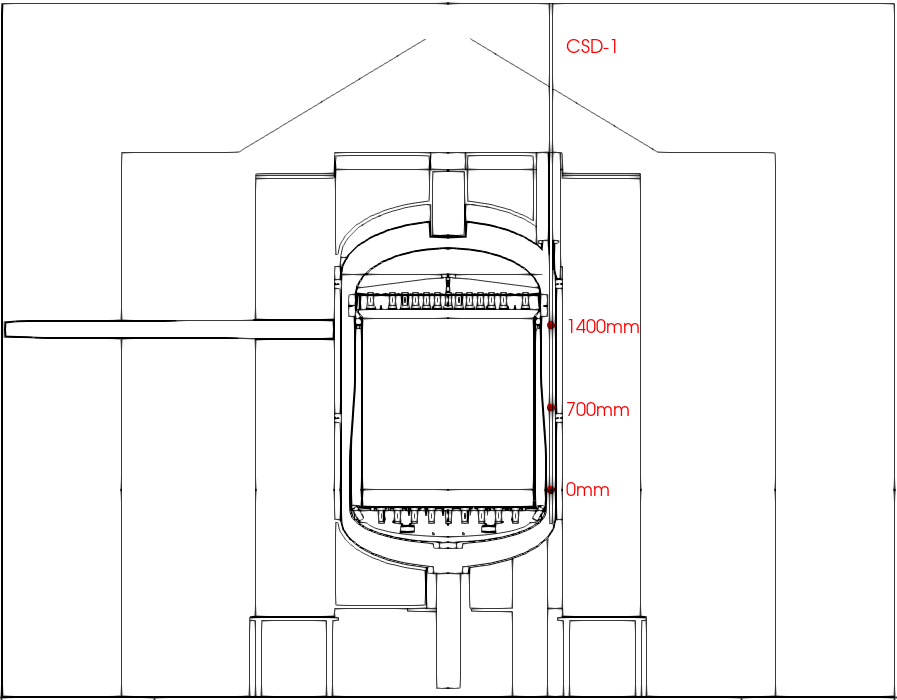
\includegraphics[width=\textwidth]{Figures/Geometry/csd1_geometry_black_and_white.png}
\caption{LZ geometry slice as implemented in GEANT4 from the water tank in. CSD-1 is shown along with the relevant Z-positions for calibration runs.}
\label{fig:CSD1_Geometry}
\end{figure}

\par
A single scatter is generally a cluster of activity close enough together that it cannot be distinguished.
The result from LUX \cite{lux_position_reconstruction_ref}, scaled to LZ as per \cite{LZ_TechnicalDesignReview_ref} give a definition of a single scatter as ${\sigma}_{z}<0.3$cm and ${\sigma}_{r}<3.0$cm.
The \textbf{SS} cut is defined as this.
The \textbf{FID} and skin are handled as before.
The result of the simulations are shown in Figure \ref{fig:simulated_amli_neutron_efficiency}.


\begin{figure}[!htbp]%
\centering
\begin{tikzpicture}
\centering
    \begin{groupplot}[%view={0}{90},
    group style = {group size = 3 by 1,vertical sep=1.5cm}]
    \nextgroupplot[
            xlabel=Veto Window ($\mu$s),
            ylabel=Efficiency (\%),
            width=15cm, height=6cm,
            xmin=0, xmax=1000,
            ymin=85, ymax=100,
            minor y tick num=4,
            grid=major,
            legend style = { column sep = 10pt, legend columns = -1, legend to name = Simulated_AmLi_CommonLegend,}]
            \addplot+[green, mark=none]
                    table [x=Time,y=Efficiency]
                    {Data/Neutron_Efficiency/Simulation/edep_amli_neutron_eff_amli_edeps_threshold_0kev_error_bars.dat};
            \addplot[green, only marks, mark size=2pt,
                     error bar legend,
                     error bars/.cd,
                     x dir=both, x explicit, error bar style={color=black}]
                    table [x=Time,y=Efficiency, x error=EfficiencyError]
                    {Data/Neutron_Efficiency/Simulation/edep_amli_neutron_eff_amli_edeps_threshold_0kev_error_bars.dat};
                    
            \addplot+[blue, mark=none]
                    table [x=Time,y=Efficiency]
                    {Data/Neutron_Efficiency/Simulation/edep_amli_neutron_eff_amli_edeps_threshold_100kev_error_bars.dat};
            \addplot[blue, only marks, mark size=2pt,
                     error bar legend,
                     error bars/.cd,
                     x dir=both, x explicit, error bar style={color=black}]
                    table [x=Time,y=Efficiency, x error=EfficiencyError]
                    {Data/Neutron_Efficiency/Simulation/edep_amli_neutron_eff_amli_edeps_threshold_100kev_error_bars.dat};
                    
            \addplot+[red, mark=none]
                    table [x=Time,y=Efficiency]
                    {Data/Neutron_Efficiency/Simulation/edep_amli_neutron_eff_amli_edeps_threshold_200kev_error_bars.dat};
            \addplot[red, only marks, mark size=2pt,
                     error bar legend,
                     error bars/.cd,
                     x dir=both, x explicit, error bar style={color=black}]
                    table [x=Time,y=Efficiency, x error=EfficiencyError]
                    {Data/Neutron_Efficiency/Simulation/edep_amli_neutron_eff_amli_edeps_threshold_200kev_error_bars.dat};
            \legend{,0keV,,100keV,,200keV}
        \nextgroupplot[group/empty plot]
        
        \nextgroupplot[group/empty plot]
        
    \end{groupplot}
     \node at ($(group c1r1) + (-0.5cm, 3.0cm)$) {\ref{Simulated_AmLi_CommonLegend}};
\end{tikzpicture}
    \caption{Simulated AmLi neutron tagging efficiency}
    \label{fig:simulated_amli_neutron_efficiency}
\end{figure}


\begin{figure}
    \centering
    
\includegraphics[width=0.5\textwidth]{Figures/Placeholder.png}
    \caption{Neutron capture time in the GdLS for AmLi events.}
    \label{fig:simulated_amli_capture_time}
\end{figure}

\begin{figure}
    \centering
    
\includegraphics[width=0.5\textwidth]{Figures/Placeholder.png}
    \caption{Neutron capture time in the GdLS from AmLi CSD-1 700mm depending upon volume the neutron spent time in.}
    \label{fig:simulated_neutron_capture_time_vs_volume}
\end{figure}



\par
In addition to the
Additionally, during the calibration data taking it will not be possible to have such ideal circumstances to test the neutron tagging performance.
Therefore, in order to quantify this, two neutron sources were simulated, AmLi and DD, the deployment methods of each are described in Section XXX.


Particularly given the propagation effects raised in Section XXX.
\par
In Chapter \ref{chap:analysis_of_the_od}, the requirements are tested in data.

\begin{table}[!htbp]
    \centering
    \begin{tabular}{c|c|c|c|c|c|c}
         \multirow{2}{*}{Neutron Source} & \multicolumn{5}{c|}{Number passing cut}      & \multirow{2}{*}{Veto Eff. (\%)}  \\ 
                         & Simulated  & Usable     & SS        & FID     & Veto         &                                  \\ \hline
        energy dep       & 19,310,000 & 19,280,766 & 1,474,033 & 325,080 & 323,319      & 99.4                             \\
        1400mm ede       & 19,310,000 & 19,280,766 & 1,474,033 & 325,080 & 323,319      & 99.4                             \\
        700mm edep       & 19,310,000 & 19,280,766 & 1,474,033 & 325,080 & 323,319      & 99.4                             \\
        0mm edep         & 19,310,000 & 19,280,766 & 1,474,033 & 325,080 & 323,319      & 99.4                             \\
        700mm optical    & X          & X          &           &         &              & 
    \end{tabular}
    \caption{Number of events passing various cuts from AmLi simulation in CSD-1.}
    \label{tab:amli_neutron_simulations_veto_efficiency}
\end{table}



\begin{figure}[!htbp]%
\centering
\begin{tikzpicture}
\centering
    \begin{axis}[
            xlabel=Energy (MeV),
            ylabel=Probability,
            width=15cm,
            height=6cm,
            grid=major,
            xmin=0, xmax=1000,
            ymin=85, ymax=100,
            %legend style={at={(50.0,9.0)},anchor=north west},
            ]
            \addplot+[green, mark=none]
                    table [x=Time,y=Efficiency]
                    {Data/Neutron_Efficiency/Simulation/amli_neutron_eff_0kev_error_bars.dat};
            \addplot[green, only marks, mark size=2pt,
                     error bar legend,
                     error bars/.cd,
                     x dir=both, x explicit, error bar style={color=black}]
                    table [x=Time,y=Efficiency, x error=EfficiencyError]
                    {Data/Neutron_Efficiency/Simulation/amli_neutron_eff_0kev_error_bars.dat};
            \addplot+[blue, mark=none]
                    table [x=Time,y=Efficiency]
                    {Data/Neutron_Efficiency/Simulation/amli_neutron_eff_50kev_error_bars.dat};
            \addplot[blue, only marks, mark size=2pt,
                     error bar legend,
                     error bars/.cd,
                     x dir=both, x explicit, error bar style={color=black}]
                    table [x=Time,y=Efficiency, x error=EfficiencyError]
                    {Data/Neutron_Efficiency/Simulation/amli_neutron_eff_50kev_error_bars.dat};
            \addplot+[red, mark=none]
                    table [x=Time,y=Efficiency]
                    {Data/Neutron_Efficiency/Simulation/amli_neutron_eff_100kev_error_bars.dat};
            \addplot[red, only marks, mark size=2pt,
                     error bar legend,
                     error bars/.cd,
                     x dir=both, x explicit, error bar style={color=black}]
                    table [x=Time,y=Efficiency, x error=EfficiencyError]
                    {Data/Neutron_Efficiency/Simulation/amli_neutron_eff_100kev_error_bars.dat};
            \legend{,0keV,,100keV,,200keV}
            \end{axis}
\end{tikzpicture}
    \caption{Simulated AmLi neutron tagging efficiency for CSD-1 at 700mm.}
    \label{fig:simulated_amli_neutron_efficiency.}
\end{figure}

